% !TEX encoding = UTF-8 Unicode

\section{Características gerais}

\subsection{Organização da memória}

O ambiente de execução da MVN fornece aos programadores um tamanho limitado de memória para ser usado no geral, a ser compartilhado entre o código e as variáveis do programa. O montador aloca a memória com base nos endereços relativos especificados no código do programa. Do total, a parte inicial da memória é reservada para guardar as instruções que serão executadas pelo programa. A parte final da memória deve ser usada especialmente para o uso do registro de ativação.

De maneira mais objetiva, reserva-se uma parte do código para a área de dados, uma parte para a função principal e as subrotinas e uma parte dedicada a pilhas de variáveis e endereços que viabilizam a chamada de subrotinas.

\subsection{Registro de ativação}

As funções em programas têm variáveis locais, que devem ser criadas na chamada da função e sobrevivem até que a função retorne. Elas também possuem recursão, onde cada instância da função tem seus próprios parâmetros e locais. As chamadas de funções se comportam de maneira LIFO, portanto podemos usar uma pilha como estrutura.

As operações push e pop dessa pilha não podem ser feitas individualmente para cada variável. Desa forma, manipula-se conjuntos de variáveis, e precisamos ter acesso a todas elas. Com isso, definimos dois conceitos:

\begin{itemize}
	\item \emph{Stack Pointer} (SP):
	\begin{itemize}
		\item Todas as posições além do SP são lixo;
		\item Todas as anteriores estão alocadas.
	\end{itemize}
	
	\item \emph{Activation Record} ou \emph{Stack Frame}
	\begin{itemize}
		\item área na pilha reservada para os dados de uma função (parâmetros, locais, endereço de retorno, etc).
                \item esta parte da pilha foi fusionada à parte anterior,
                    facilitando o uso da pilha e diminuindo a quantidade de
                    dados na mesma. Esta decisão não afeta a implantação, uma
                    vez que no caso desta linguagem o compilador tem total
                    controle do tamanho das estruturas sendo utilizadas. 
	\end{itemize}
\end{itemize}

\begin{figure}[ht]
	\centering
	\caption{Esquema do Registro de Ativação}
	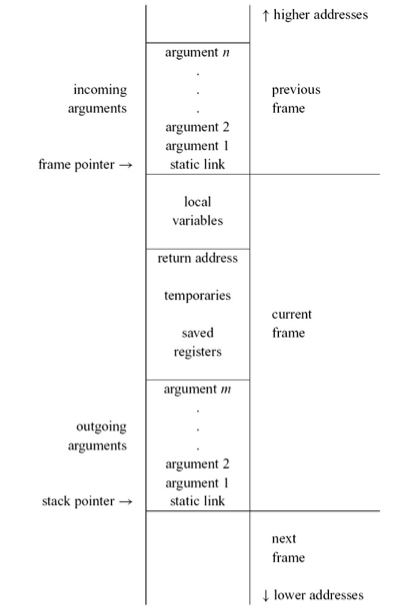
\includegraphics[width=0.5\textwidth]{images/registros-ativacao.png}
	\label{fig:registros-ativacao}
\end{figure}

A figura~\ref{fig:registros-ativacao} ilustra a organização da pilha. O uso do registro de ativação permite entre outras coisas a chamada recursiva de funções, uma vez isso não é possível de forma nativa no ambiente da MVN. No caso da MVN, a pilha cresce para baixo e as subrotinas são executadas utilizando as seguintes instruções:

\begin{itemize}
	\item Desvio para subprograma - mnemônico SC (0xA): armazena o endereço de instrução seguinte (atual + 1) na posição de memória apontada pelo operando. Em seguida, desvia a execução para o endereço indicado pelo operando e acrescido de uma unidade.
	
	\item Retorno de subprograma - mnemônico RS (0xB): desvia a execução para o endereço indicado pelo valor guardado na posição de memória do operando.
\end{itemize}

Foi criada por nós uma biblioteca em assembly para implementar funções auxiliares de entrada e saída de dados, além da funcionalidade de empilhar, desempilhar e ter acesso a informações contidas na pilha discutida anteriormente. Essas funções são explicadas na próxima seção.

\section{Biblioteca desenvolvida em Assembly}

A biblioteca padrão desenvolvida é dividida em dois módulos o primeiro
implementa as funções básicas de empilhamento, sendo chamado de \verb!std.asm!.
O segundo módulo implementa as operações de input e output de dados, de nome 
\verb!stdio.asm!.

\subsection{STD}

A manipulação de pilhas é feita pela biblioteca padrão, sendo que deseja-se
seguir a estrutura abaixo definida, facilitando o uso e acesso das variáveis.
Vemos abaixo um exemplo do uso da biblioteca. Na linha 23 salvamos uma variável
recebida por parâmetro na pilha e na linha 30 recuperamos seu valor. 

Logo antes de retornar devemos executar a função \verb!POP_CALL! 
ela é responsável por
escrever o endereço de retorno na função em que estamos, assim aproveitando das
chamadas existentes na \verb!MVN! (funções devem ser \emph{stateless} para tanto). Percebe-se
que é possível executar a função recursivamente (linha 55 e 57). Para tanto é
necessário chamar a função \verb!PUSH_CALL! para que a mesma efetue o
empilhamento e escreva o endereço de retorno atual na pilha. 

\begin{lstlisting}[basicstyle=\footnotesize,numbers=left,breaklines=true,morekeywords={}]
;; VARIAVEIS GLOBAIS
;; comeco da pilha = FFF 
;; tamanho da pilha = 2FF 
;;   | ptr to old_stack_head  | \___ STACK_PTR
;;   |      savedregist       |   
;;   |         ...            |   
;;   |      local var         |  
;;   |         ...            |   
;;   |      temporaries       |  
;;   |      parameters        |   
;;   |         ...            |  
;;   |     ref parameters     |  ____ OLD STACK_PTR
;;   |      returnaddrs       | /     (STACK_PTR points here)

EXAMPLE_STACK_ARG    K  /0000
EXAMPLE_STACK        JP /000 
                     SC PRINT_STACK_ADDRS   ;; deve imprimir 0fff 
                     ;;; SALVAR ARGUMENTOS na pilha 
                     LV =0
                     MM WORD_TO_SAVE 
                     LV EXAMPLE_STACK_ARG 
                     MM ORIGIN_PTR 
                     SC SAVE_WORD_TO_LOCAL_VAR 
                     ;;;; CORPO DA FUNCAO 
                     ;;; CARREGANDO UM VALOR DA PILHA 
                     LV =0
                     MM WORD_TO_GET 
                     LV EXAMPLE_STACK_ARG 
                     MM STORE_PTR
                     SC GET_WORD_LOCAL_VAR 
                     ;;; IMPRIME 
                     LV COUNT_IS
                     MM STRING_PTR 
                     SC P_STRING  ;; inline fct, no need to stack 
                     LD EXAMPLE_STACK_ARG 
                     MM TO_BE_PRINTED 
                     SC P_INT_ZERO
                     SC P_LINE

                     LD EXAMPLE_STACK_ARG
                     JZ RETURN_EXAMPLE_STACK

                     LD EXAMPLE_STACK_ARG 
                     -  ONE 
                     MM EXAMPLE_STACK_ARG 

                     LV =1
                     MM PUSH_CALL_SIZELV
                     LV =0
                     MM PUSH_CALL_RET_ADDRS 
                     LV =0
                     MM PUSH_CALL_TMP_SZ
                     LV =0
                     MM PUSH_CALL_PAR_SZ 
                     SC PUSH_CALL

                     SC EXAMPLE_STACK  ;; chamada recursiva
                     ;;;; FIM DO CORPO DA FUNCAO 
RETURN_EXAMPLE_STACK LV EXAMPLE_STACK
                     MM POP_CALL_FCT 
                     SC POP_CALL ;; trickery!

                     SC PRINT_STACK_ADDRS   ;; deve imprimir 0fff 
                     RS EXAMPLE_STACK
\end{lstlisting}

Abaixo podemos ver a implementação das funções de \verb!PUSH! e \verb!POP!

A pilha é implementada dos valores mais altos da memória para os valores mais
baixos, sendo assim, o ponteiro de pilha começa apontando para \verb!0x0FFF!.

A pilha funciona como uma lista ligada que guarda o endereço da última célula
da pilha. Sendo assim, a operação de \verb!POP! é trivial. Estas funções fazem
a gestão do endereço de retorno automaticamente, contanto que se siga a
premissa de chamada (chamada da função logo após a chamada de \verb!PUSH_CALL!
e seus parâmetros).

\begin{lstlisting}[basicstyle=\footnotesize,numbers=left,breaklines=true,morekeywords={}]
;; *** PUSH_CALL ***
PUSH_CALL           JP /000 
                    LD PUSH_CALL  ;; get return addrs 
                    +  TWO ;; return address of the callee
                    +  LOADV_CONST
                    MM LOAD_RETURN_ADDRS 
                    LD STACK_PTR
                    -  TWO        ;; new return addrs  
                    +  MOVE_CONST 
                    MM MOVE_RETURN_ADDRS 
LOAD_RETURN_ADDRS   JP /000  
MOVE_RETURN_ADDRS   JP /000   ;; return addrs salvo 
                    LD STACK_PTR          
                    -  TWO 
                    -  TWO 
                    -  PUSH_CALL_SIZELV
                    -  PUSH_CALL_RET_ADDRS
                    -  PUSH_CALL_TMP_SZ
                    -  PUSH_CALL_PAR_SZ 
                    -  TWO  ;; return addrs
                    MM TMP_1
                    LD TMP_1 
                    +  MOVE_CONST 
                    MM MRKR_PC_SAVE_HEAD 
                    LD STACK_PTR 
MRKR_PC_SAVE_HEAD   JP /000 
                    LD TMP_1 
                    MM STACK_PTR
                    RS PUSH_CALL
;; **** POP_CALL ****

POP_CALL_FCT        K /0000             
POP_CALL            JP /000 ; retorno 
POP_CALL_INIT       LD STACK_PTR 
                    +  LOAD_CONST 
                    MM MRKR_PC_LOAD_HEAD 
MRKR_PC_LOAD_HEAD   JP /000 
                    MM STACK_PTR 
                    LD STACK_PTR 
                    -  TWO
                    +  LOAD_CONST 
                    MM LOAD_RETURN_ADDRS_2
                    LD POP_CALL_FCT 
                    +  MOVE_CONST 
                    MM MOVE_RETURN_ADDRS_2
LOAD_RETURN_ADDRS_2 JP /000 
MOVE_RETURN_ADDRS_2 JP /000  ;; engana a funcao para ela pensar que ela 
                             ;; tem que retornar para esse valor 
                    RS POP_CALL
\end{lstlisting}


As rotinas de salvaguarda e carregamento dos valores locais, parâmetros,
   referências pode ser feita por meio das chamadas abaixo, 
   \verb!SAVE_WORD_TO_LOCAL_VAR! e \verb!GET_WORD_LOCAL_VAR! respectivamente.

\begin{lstlisting}[basicstyle=\footnotesize,numbers=left,breaklines=true,morekeywords={}]
;; **** SAVE_WORD_TO_LOCAL_VAR WORD_TO_SAVE ORIGIN_PTR ****
SAVE_WORD_TO_LOCAL_VAR      JP /000 
                            LD STACK_PTR
                            + TWO          ;; first word 
                            + WORD_TO_SAVE 
                            + WORD_TO_SAVE  ;; WORD_TO_GET * 2
                            + MOVE_CONST   ;; 
                            MM MOVE_WORD_LOCAL_VAR_2
                            LD ORIGIN_PTR
                            + LOAD_CONST 
                            MM LOAD_WORD_LOCAL_VAR_2
LOAD_WORD_LOCAL_VAR_2       JP /000 ;; 8FROMPTR
MOVE_WORD_LOCAL_VAR_2       JP /000 ;; 9TOPTR
                            RS SAVE_WORD_TO_LOCAL_VAR

;; **** GET_WORD_LOCAL_VAR WORD_TO_GET STORE_PTR ****


WORD_TO_GET        K /000 
STORE_PTR          K /000

GET_WORD_LOCAL_VAR          JP /000 
                            LD STACK_PTR
                            + TWO          ;; first word 
                            + WORD_TO_GET  
                            + WORD_TO_GET  ;; WORD_TO_GET * 2
                            + LOAD_CONST   ;; 
                            MM LOAD_WORD_LOCAL_VAR  
                            LD STORE_PTR
                            + MOVE_CONST 
                            MM MOVE_WORD_LOCAL_VAR
LOAD_WORD_LOCAL_VAR         JP /000 ;; 8FROMPTR
MOVE_WORD_LOCAL_VAR         JP /000 ;; 9TOPTR
                            RS GET_WORD_LOCAL_VAR
 \end{lstlisting}


\subsection{STDIO}


O ambiente de execução também é provido de funções de input/output:

Para a impressão de \emph{strings} podemos utilizar a função \verb!P_STRING!, 
     passando o ponteiro para o começo de uma \verb!string!. Em \verb!CZAR!
     consideramos \emph{strings} como sendo \emph{bytes} em um vetor de
     \emph{word} terminados pelo \emph{byte} \verb!0x0000!. Vale salientar que
     esta forma de armazenamento não causa problemas com outros tipos de
     armazenamento mais compactos, como a utilização dos dois \emph{bytes}
     da \emph{word} para armazenamento de \emph{chars} subsequentes. Quando a
     função recebe a \emph{word} \verb!0x0030!, primeiramente ela vai imprimir
     \verb!0x00! que é o caractere nulo, portanto, sem impressão e então
     imprimir o caractere correspondente a \verb!0x30!. 

\begin{lstlisting}[basicstyle=\footnotesize,numbers=left,breaklines=true,morekeywords={}]
;; ****  P_STRING &STRING_PTR ****
;;   Imprime a string apontada por STRING_PTR ate
;; o caractere /000  

P_STRING            JP /000           ; endereco de retorno 
PSTRINGINIT         LD STRING_PTR 
                    MM TO_BE_PRINTED_TMP 
LOAD_TO_BE_PRINTED  LD TO_BE_PRINTED_TMP
                    +  LOAD_CONST    
                    MM LABELLOAD 
LABELLOAD           K  /0000 
                    JZ P_STRING_END  ; se zero vamos para o final!
                    PD /100 
                    LD TO_BE_PRINTED_TMP
                    +  TWO
                    MM TO_BE_PRINTED_TMP
                    JP LOAD_TO_BE_PRINTED
P_STRING_END        RS P_STRING 

 \end{lstlisting}

Para a leitura de \emph{strings} seguimos o padrão definido anteriormente, um
\emph{byte} (\emph{char}) por \emph{word}:

\begin{lstlisting}[basicstyle=\footnotesize,numbers=left,breaklines=true,morekeywords={}]
;; *** GETS STORE_PTR_IO ***
;; Existe um problema de buffer aqui... nao vamos 
;; trata-lo, pois este e' um problema intri'nseco da 
;; MVN. (leitura e subsequente bloqueio por word)
LAST_CONTROL_CHAR_P_ONE    K /0021
ARRAY_POS_BYTE  JP /000
GETS            JP /000
                LD STORE_PTR_IO
                MM ARRAY_POS_BYTE
GETS_LOOP       GD /000
                MM HIGH_V
                SC HIGH_LOW 
                LD HIGH_V 
                -  LAST_CONTROL_CHAR_P_ONE 
                JN RETURN_GETS 
                LD ARRAY_POS_BYTE 
                +  MOVE_CONST 
                MM MOVE_HIGH_V
                LD HIGH_V 
MOVE_HIGH_V     JP /000 

                LD ARRAY_POS_BYTE
                +  TWO 
                MM ARRAY_POS_BYTE 

                LD LOW_V 
                -  LAST_CONTROL_CHAR_P_ONE 
                JN RETURN_GETS 
                LD ARRAY_POS_BYTE 
                +  MOVE_CONST 
                MM MOVE_LOW_V
                LD LOW_V 
MOVE_LOW_V      JP /000 

                LD ARRAY_POS_BYTE
                +  TWO 
                MM ARRAY_POS_BYTE 

                JP GETS_LOOP 

RETURN_GETS     LD ARRAY_POS_BYTE 
                +  MOVE_CONST 
                MM MOVE_ZERO
                LV =000  
MOVE_ZERO       JP /000 

                LD ARRAY_POS_BYTE
                +  TWO 
                MM ARRAY_POS_BYTE 
                RS GETS

\end{lstlisting}

A biblioteca também é capaz de realizar a leitura e escrita de valores
inteiros (funções auxiliares estão disponíveis no pacote em anexo): 

\begin{lstlisting}[basicstyle=\footnotesize,numbers=left,breaklines=true,morekeywords={}]
;; *** READ_INT STORE_PTR_IO ***
;; doesnt care about buffers, should have a trailing char at the end of the
;; stream otherwise it will just discard it.. 
STORE_PTR_IO        JP /000
ZERO_M_ONE          K  /002F
NINE_P_ONE          K  /0039

LOW                 K  /0000
HIGH                K  /0000
GO_IF_NUMBER        K  /0000 
TO_BE_TRIMMED       K  /0000 
TBT_TMP             K  /0000 

TRIM_INT            JP /000
                    LD TO_BE_TRIMMED
                    /  SHIFT_BYTE  
                    *  SHIFT_BYTE
                    MM TBT_TMP 
                    LD TO_BE_TRIMMED
                    -  TBT_TMP 
                    MM TO_BE_TRIMMED 
                    RS TRIM_INT 

READ_INT_WORD       JP /000
                    GD /000 
                    MM TMP_3 
                    LD TMP_3
                    /  SHIFT_BYTE
                    MM TO_BE_TRIMMED 
                    SC TRIM_INT 
                    LD TO_BE_TRIMMED
                    MM HIGH 

                    LD TMP_3
                    MM TO_BE_TRIMMED 
                    SC TRIM_INT
                    LD TO_BE_TRIMMED
                    MM LOW
                    RS READ_INT_WORD

READ_INT            JP /000 
                    LV =0 
                    MM TMP_4
READ_INT_LOOP       SC READ_INT_WORD 
                    LD HIGH 
                    MM TMP_3 
                    LV CONT1
                    MM GO_IF_NUMBER
                    JP IF_NUMBER_CONTINUE 
CONT1               LD LOW
                    MM TMP_3 
                    LV READ_INT_LOOP
                    MM GO_IF_NUMBER
                    JP IF_NUMBER_CONTINUE 
NOT_NUMBER          LD STORE_PTR_IO
                    +  MOVE_CONST 
                    MM MOVE_READ_INT
                    LD TMP_4 
MOVE_READ_INT       JP /000
                    RS READ_INT 

IF_NUMBER_CONTINUE  LD TMP_3 
                    -  ZERO_M_ONE 
                    JN NOT_NUMBER 
                    LD NINE_P_ONE 
                    -  TMP_3
                    JN NOT_NUMBER  

                    LD TMP_4
                    *  TEN 
                    MM TMP_4 


                    LD TMP_3 
                    -  ZERO_M_ONE
                    -  ONE 
                    +  TMP_4
                    MM TMP_4

                    LD GO_IF_NUMBER
                    MM END_READ_INT
END_READ_INT        JP /000
\end{lstlisting}

A impressão de inteiros, por ser crítica e muito importante para a correção de
erros, foi feita de forma simples e direta. Sem laços (unwind de \verb!GOTO!
    explícito) ou complicações,
    resultando em uma função bem determinada e robusta.
\begin{lstlisting}[basicstyle=\footnotesize,numbers=left,breaklines=true,morekeywords={}]
;; *** P_INT_ZERO TO_BE_PRINTED ***
;;  Imprime um inteiro (com zeros a esquerda)
;; ex:  
;;  INT_2 K  =345 
;;        LD INT_2
;;        MM TO_BE_PRINTED 
;;        SC P_INT_ZERO
;; imprime 00345
;;
;;
;; Esta funcao esta com o loop inline
;; sendo simples e robusta

P_INT_ZERO          JP /000
P_INT_INIT          JP P_INT_REAL_INIT
ZERO_BASE           K /30
;; bases para a conversao:
INT_POT_1           K =10000   
INT_POT_2           K =1000 
INT_POT_3           K =100  
INT_POT_4           K =10 
INT_POT_5           K =1 
P_INT_REAL_INIT     LD TO_BE_PRINTED       ;; PRIMEIRO CHAR
                    MM TMP_1 
                    /  INT_POT_1 
                    +  ZERO_BASE 
                    PD /100                     ;; imprime 
                    LD TMP_1  
                    /  INT_POT_1
                    *  INT_POT_1 
                    MM TMP_2                     
                    LD TMP_1
                    -  TMP_2
                    MM TMP_1   
                    /  INT_POT_2                ;; segundo char 
                    +  ZERO_BASE 
                    PD /100                     ;; imprime 
                    LD TMP_1  
                    /  INT_POT_2
                    *  INT_POT_2 
                    MM TMP_2                     
                    LD TMP_1
                    -  TMP_2
                    MM TMP_1 
                    /  INT_POT_3                ;; terceiro char 
                    +  ZERO_BASE 
                    PD /100                     ;; imprime 
                    LD TMP_1  
                    /  INT_POT_3
                    *  INT_POT_3 
                    MM TMP_2                     
                    LD TMP_1
                    -  TMP_2
                    MM TMP_1 
                    /  INT_POT_4                ;; quarto char 
                    +  ZERO_BASE 
                    PD /100                     ;; imprime 
                    LD TMP_1  
                    /  INT_POT_4
                    *  INT_POT_4 
                    MM TMP_2                     
                    LD TMP_1
                    -  TMP_2
                    MM TMP_1 
                    /  INT_POT_5                ;; quinto char 
                    +  ZERO_BASE 
                    PD /100                     ;; imprime 
                    LD TMP_1  
                    /  INT_POT_5
                    *  INT_POT_5 
                    MM TMP_2                     
                    LD TMP_1
                    -  TMP_2
                    MM TMP_1 
                    RS P_INT_ZERO

 \end{lstlisting}

